\begin{figure}[htbp]
\section*{ NIPBL}
\centering
\begin{subfigure}[b]{0.95\textwidth}
\centering
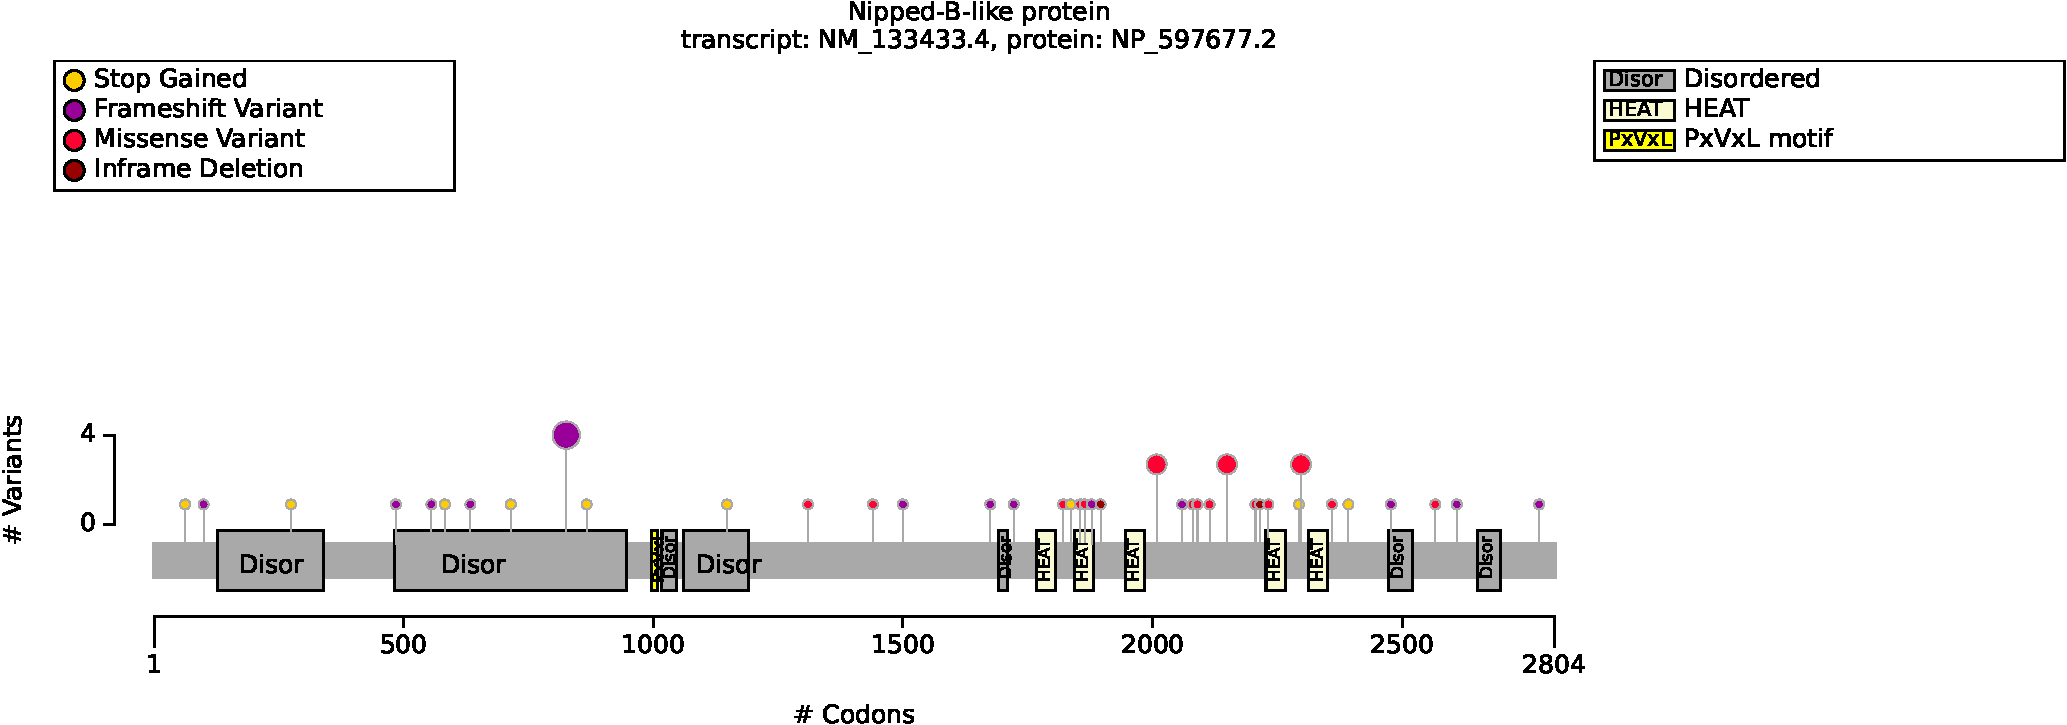
\includegraphics[width=\textwidth]{ img/NIPBL_protein_diagram.pdf} 
\captionsetup{justification=raggedright,singlelinecheck=false}
\caption{Distribution of variants in NIPBL}
\end{subfigure}

\vspace{2em}

\begin{subfigure}[b]{0.95\textwidth}
\centering
\resizebox{\textwidth}{!}{
\begin{tabular}{llllrr}
\toprule
Genotype (A) & Genotype (B) & total tests performed & significant results\\
\midrule
missense & other & 86 & 0\\
disordered & other & 86 & 0\\
FEMALE & MALE & 81 & 0\\
\bottomrule
\end{tabular}
}
\captionsetup{justification=raggedright,singlelinecheck=false}
\caption{             Fisher Exact Test performed to compare HPO annotation frequency with respect to genotypes. }
\end{subfigure}

\vspace{2em}

\caption{ The cohort comprised 60 individuals (21 females, 31 males, 8 with unknown sex). A total of 90 HPO terms were used to annotate the cohort. Disease diagnosis: Cornelia de Lange syndrome 1 (OMIM:122470). No statistically significant genotype-phenotype correlation identified. A total of 50 unique variant alleles were found in \textit{NIPBL} (transcript: \texttt{NM\_133433.4}, protein id: \texttt{NP\_597677.2}).}
\end{figure}
